\documentclass[12pt,oneside]{uhthesis}
\usepackage{subfigure}
\usepackage[ruled,lined,linesnumbered,titlenumbered,algochapter,spanish,onelanguage]{algorithm2e}
\usepackage{amsmath}
\usepackage{amssymb}
\usepackage{amsbsy}
\usepackage{caption,booktabs}
\captionsetup{ justification = centering }
%\usepackage{mathpazo}
\usepackage{float}
\setlength{\marginparwidth}{2cm}
\usepackage{todonotes}
\usepackage{listings}
\usepackage{xcolor}
\usepackage{multicol}
\usepackage{graphicx}
\floatstyle{plaintop}
\restylefloat{table}
\addbibresource{Bibliography.bib}
% \setlength{\parskip}{\baselineskip}%
\renewcommand{\tablename}{Tabla}
\renewcommand{\listalgorithmcfname}{Índice de Algoritmos}
%\dontprintsemicolon
\SetAlgoNoEnd

\definecolor{codegreen}{rgb}{0,0.6,0}
\definecolor{codegray}{rgb}{0.5,0.5,0.5}
\definecolor{codepurple}{rgb}{0.58,0,0.82}
\definecolor{backcolour}{rgb}{0.95,0.95,0.92}

\lstdefinestyle{mystyle}{
    backgroundcolor=\color{backcolour},   
    commentstyle=\color{codegreen},
    keywordstyle=\color{purple},
    numberstyle=\tiny\color{codegray},
    stringstyle=\color{codepurple},
    basicstyle=\ttfamily\footnotesize,
    breakatwhitespace=false,         
    breaklines=true,                 
    captionpos=b,                    
    keepspaces=true,                 
    numbers=left,                    
    numbersep=5pt,                  
    showspaces=false,                
    showstringspaces=false,
    showtabs=false,                  
    tabsize=4
}

\lstset{style=mystyle}

\title{Título de la tesis}
\author{\\\vspace{0.25cm}Nombre del autor}
\advisor{\\\vspace{0.25cm}Nombre del primer tutor\\\vspace{0.2cm}Nombre del segundo tutor}
\degree{Licenciado en (Matemática o Ciencia de la Computación)}
\faculty{Facultad de Matemática y Computación}
\date{Fecha\\\vspace{0.25cm}\href{https://github.com/username/repo}{github.com/username/repo}}
\logo{Graphics/uhlogo}
\makenomenclature

\renewcommand{\vec}[1]{\boldsymbol{#1}}
\newcommand{\diff}[1]{\ensuremath{\mathrm{d}#1}}
\newcommand{\me}[1]{\mathrm{e}^{#1}}
\newcommand{\pf}{\mathfrak{p}}
\newcommand{\qf}{\mathfrak{q}}
%\newcommand{\kf}{\mathfrak{k}}
\newcommand{\kt}{\mathtt{k}}
\newcommand{\mf}{\mathfrak{m}}
\newcommand{\hf}{\mathfrak{h}}
\newcommand{\fac}{\mathrm{fac}}
\newcommand{\maxx}[1]{\max\left\{ #1 \right\} }
\newcommand{\minn}[1]{\min\left\{ #1 \right\} }
\newcommand{\lldpcf}{1.25}
\newcommand{\nnorm}[1]{\left\lvert #1 \right\rvert }
\renewcommand{\lstlistingname}{Ejemplo de código}
\renewcommand{\lstlistlistingname}{Ejemplos de código}

\begin{document}

\frontmatter
\maketitle

\begin{dedication}
    Dedicación
\end{dedication}
\begin{acknowledgements}
    En primer lugar, quiero agradecer a mi familia, que siempre me brindó todo su apoyo; en especial, a las cinco personas que han estado más presentes: mi madre, mi tía Hosy, mi primo (casi como un hermano) Marcelo, mi abuela Mery y mi abuelo Andrés, quienes me acompañaron durante este largo proceso de superación personal y nunca permitieron que me faltara nada. También agradezco a mi padre y a mi madrastra Mariela, quienes, a pesar de la distancia, mostraron interés y preocupación por mi progreso.

    También quisiera agradecer a mis compañeros Max, David, Jorge, José, Yoan, Alex, Ovidio, Davier, entre otros que quizás olvido mencionar y pido disculpas por ello, por toda la ayuda que me brindaron en las etapas más difíciles de cada semestre.

    A mi pareja Lía, por haber sido tan comprensiva cuando he tenido que volcarme completamente en los estudios.

    Al profe Frank Fonseca, por haberme brindado las herramientas para poder terminar este trabajo y haber sido paciente en su tutela, a pesar de los contratiempos que a menudo se me presentaban.

    Por último, pero no menos importante, un agradecimiento enorme a William \\ Headrick, quien, no conforme con ayudarme a mejorar mi dominio del inglés de forma totalmente desinteresada, también constituyó un pilar económico para mi etapa universitaria en el momento en que más mi familia y yo lo necesitábamos.
\end{acknowledgements}

\begin{opinion}
    Opiniones de los tutores
\end{opinion}
\begin{resumen}
	Esta tesis presenta una infraestructura de clave pública (PKI) integrada con Hyperledger Fabric para la autenticación segura de nodos en una red blockchain. Se ha desarrollado una Autoridad Certificadora (CA) propia mediante una API en Node.js, que permite la gestión eficiente de identidades y la emisión automatizada de certificados mediante OpenSSL. Hyperledger Fabric, al ser una plataforma modular y permisionada, ofrece herramientas avanzadas para la administración de identidades a través de Membership Service Providers (MSP) y la segmentación de datos mediante canales privados. La solución implementada aprovecha estas características, automatizando la configuración de la red a partir de archivos YAML y utilizando scripts en Bash para la generación del bloque génesis y el despliegue en Docker. Los resultados muestran mejoras en la seguridad, escalabilidad y gestión de identidades, optimizando la incorporación de nodos en la red y permitiendo una mayor flexibilidad en la configuración. Se proponen futuras mejoras, como la integración de bases de datos para la gestión de certificados y la implementación de herramientas de monitoreo.
	
\end{resumen}

\begin{abstract}
	This thesis presents a public key infrastructure (PKI) integrated with Hyperledger Fabric for secure node authentication in a blockchain network. A custom Certificate Authority (CA) was developed using a Node.js API, enabling efficient identity management and automated certificate issuance via OpenSSL. Hyperledger Fabric, as a modular and permissioned platform, provides advanced tools for identity management through Membership Service Providers (MSP) and data segmentation via private channels. The implemented solution leverages these features by automating network configuration through YAML files and using Bash scripts for genesis block generation and Docker deployment. The results demonstrate improvements in security, scalability, and identity management, optimizing node onboarding and providing greater flexibility in network configuration. Future enhancements include integrating databases for certificate management and implementing monitoring tools.
	
\end{abstract}
\tableofcontents
\listoffigures
% \listoftables
% \listofalgorithms
\lstlistoflistings

\mainmatter

\chapter*{Introducción}\label{chapter:introduction}
\addcontentsline{toc}{chapter}{Introducción}

En un mundo cada vez más interconectado, la seguridad de la información se ha convertido en una necesidad fundamental. La criptografía, como disciplina, juega 
un papel crucial en la protección de datos, proporcionando confidencialidad, integridad y autenticación en diversos sistemas tecnológicos. Desde la 
protección de comunicaciones personales hasta el aseguramiento de transacciones bancarias, sus aplicaciones son amplias y esenciales para el desarrollo de un entorno 
digital confiable. Dos de las tecnologías que fundamentan su seguridad son las \textbf{infraestructuras de clave pública} (\textit{PKI}) y la \textbf{\textit{blockchain}}.

Una de las principales ventajas de las \textit{PKI} es que proporcionan \textbf{autenticación fuerte}, ya que las claves privadas son únicas para cada 
entidad y solo estas pueden ser utilizadas para firmar o cifrar datos. Además, la \textbf{integridad de los datos} se asegura mediante el uso de firmas 
digitales, garantizando que los mensajes no sean alterados durante su transmisión. Otro beneficio clave de las \textit{PKI} es su capacidad para manejar grandes volúmenes 
de certificados y claves a través de un sistema organizado de autoridades certificadoras (\textit{CA}), lo que permite la gestión eficiente de la autenticación a gran escala.

La tecnología \textbf{\textit{blockchain}}, desde su surgimiento, también ha tenido un impacto enorme en el ámbito de la informática y las finanzas. Se caracteriza por 
su naturaleza \textbf{descentralizada}, \textbf{inmutable} y \textbf{transparente}, lo que la convierte en una solución ideal para aplicaciones que requieren registros 
seguros, auditables y verificables, como las transacciones financieras y la gestión de contratos inteligentes. \textit{Blockchain} permite a las partes interactuar de manera confiable 
sin necesidad de \textit{intermediarios}, lo cual reduce significativamente los costos y riesgos asociados a las transacciones digitales.

A pesar de representar enfoques distintos, se podría aprovechar lo mejor de ambas tecnologías a partir de la integración conjunta de las mismas. Una \textit{PKI} puede proporcionar una \textbf{autenticación robusta} 
y una \textbf{gestión eficiente de claves} para los nodos de la \textit{blockchain}, asegurando que solo los participantes legítimos puedan interactuar con la red. Aunque \textit{blockchain} asegura la integridad de los datos mediante su estructura 
descentralizada y su consenso distribuido, la identificación y verificación de los participantes de la red aún requieren mecanismos seguros, como los proporcionados por una \textit{PKI}. A través de este enfoque conjunto, la combinación de 
ambas tecnologías podría mejorar significativamente la confianza en los sistemas basados en \textit{blockchain}, especialmente en contextos donde la autenticidad de los participantes y la seguridad de las transacciones son críticos.

\section{Diseño Teórico}
\subsection*{Problema Científico}

Las redes blockchain requieren mecanismos seguros y confiables para la autenticación de nodos, evitando ataques de suplantación de identidad y mejorando la confianza en la red. Sin embargo, las soluciones tradicionales de autenticación suelen ser centralizadas o difíciles de integrar en sistemas distribuidos. 

\subsection*{Pregunta científica:} ¿Es posible implementar un mecanismo de validación confiable para los nodos de una red blockchain de Hyperledger Fabric utilizando una PKI externa?

\subsection*{Objeto de Estudio}
Infraestructura de clave pública aplicada a la redes blockchain para la autenticación segura de nodos.

\subsection*{Objetivo General}\
Diseñar e implementar una Autoridad Certificadora (CA) como mecanismo de autenticación segura de los nodos en la red Blockchain.

\subsection*{Objetivos específicos}\
\begin{enumerate}
    \item Analizar los esquemas de autenticación utilizados en redes .
    \item Diseñar una CA adaptada a las necesidades de autenticación de nodos en blockchain.
    \item Implementar la solución en un entorno de prueba utilizando herramientas de seguridad criptográfica.
    \item Evaluar el rendimiento y seguridad de la solución propuesta en comparación con otros métodos de autenticación.
\end{enumerate}

\subsection*{Campo de Acción}
La plataforma de Hyperledger Fabric

\subsection*{Hipótesis}
La implementación de una PKI en una red blockchain permitirá mejorar la seguridad y confiabilidad de la autenticación de nodos, reduciendo el riesgo de ataques de suplantación de identidad y fortaleciendo la integridad del ecosistema distribuido.

\section{Estructura del trabajo}

Esta tesis está organizada en tres capítulos principales, los cuales se describen a continuación:

\begin{itemize}
    \item \textbf{Capítulo 1: Preliminares} \\
    En este capítulo se aborda el marco teórico necesario para comprender los conceptos fundamentales sobre PKI y blockchain. El objetivo es proporcionar al lector el conocimiento necesario para entender los conceptos clave que se desarrollarán en el resto del trabajo.
    
    \item \textbf{Capítulo 2: Estado del Arte} \\
    Este capítulo presenta un informe sobre los trabajos más recientes relacionados con el tema de la tesis. Se analiza la literatura existente sobre PKI y blockchain, con especial énfasis en la integración de ambas.
    
    \item \textbf{Capítulo 3: Resultados y Discusión} \\
    En este capítulo se expone la solución propuesta, explicando en detalle cómo se lleva a cabo la implementación de la PKI para la autenticación segura de nodos en Hyperledger Fabric. Además, se realiza una discusión sobre los resultados obtenidos y su comparación con soluciones existentes.
\end{itemize}

\chapter{Preliminares}

En este capítulo se presentan los conceptos y fundamentos teóricos necesarios para comprender los temas tratados en este trabajo. 
Se abordarán las bases de la tecnología \textit{blockchain} y las infraestructuras de clave pública (\textit{PKI}), destacando su 
relevancia y características principales.

\section{Criptografía asimétrica}

La criptografía asimétrica, también conocida como criptografía de clave pública, es un paradigma de cifrado que utiliza un par de claves: una pública, que 
puede ser compartida libremente, y una privada, que debe mantenerse en secreto. Este esquema permite garantizar la confidencialidad, integridad y 
autenticación en sistemas de comunicación modernos.

El verdadero despegue de esta técnica llegó en 1977 con la creación del algoritmo RSA \cite{rivest1978method}, desarrollado por Ronald Rivest, Adi Shamir y Leonard Adleman. 
Este sistema utiliza un par de claves matemáticamente relacionadas: una clave pública, que puede ser compartida libremente, y una clave privada, que debe 
mantenerse en secreto. La clave pública cifra el mensaje, mientras que la clave privada se utiliza para descifrarlo. Este enfoque resuelve el problema 
de la distribución segura de claves y hace posible la autenticación y el intercambio seguro de información en entornos inseguros como Internet.

La criptografía de clave pública surgió como una solución a dos problemas fundamentales de la criptografía simétrica:
\begin{itemize}
  \item \textbf{Distribución de claves:} En la criptografía simétrica, la distribución de claves requiere que las partes que desean comunicarse ya compartan una clave secreta o dependan de un Centro de Distribución de Claves (KDC, por sus siglas en inglés). Según Whitfield Diffie, uno de los descubridores de la criptografía de clave pública, este enfoque comprometía la esencia misma de la criptografía: mantener el secreto total de las comunicaciones. Él argumentaba: "¿De qué servirían sistemas criptográficos impenetrables si sus usuarios debieran compartir sus claves con un KDC que podría ser comprometido?" \cite{diffie1976new}
  \item \textbf{Firmas digitales:} La criptografía debía evolucionar para ser utilizada en aplicaciones comerciales y privadas, además de las militares. Esto requería un mecanismo equivalente a las firmas en documentos en papel, que garantizara de manera verificable que un mensaje digital provenía de una persona específica.
\end{itemize}

A continuación, se describen algunos términos fundamentales relacionados con este tipo de criptografía:

\begin{itemize}
  \item \textbf{Claves asimétricas}: Un par de claves relacionadas (clave pública y clave privada) que se utilizan para operaciones complementarias como el cifrado/descifrado o la generación/verificación de firmas.
  \item \textbf{Certificado de clave pública}: Un documento digital emitido y firmado por una Autoridad de Certificación (CA) que vincula el nombre de un usuario con su clave pública y confirma que solo el titular tiene acceso a la clave privada correspondiente.
  \item \textbf{Algoritmo criptográfico de clave pública}: Un algoritmo que emplea un par de claves asimétricas. La derivación de la clave privada a partir de la pública debe ser computacionalmente inviable.
  \item \textbf{Infraestructura de Clave Pública}: Conjunto de políticas, procesos, servidores, software y equipos utilizados para administrar certificados digitales y pares de claves públicas/privadas. Esto incluye la emisión, el mantenimiento y la revocación de certificados.
  \item \textbf{Llaves pública y privada}: Estas forman un par de llaves seleccionadas para que si una se utiliza para cifrar, la otra pueda descifrar. Las transformaciones realizadas dependen de cuál de las llaves (pública o privada) se utiliza como entrada.
  \item \textbf{Texto cifrado (Ciphertext)}: Es el mensaje cifrado que se produce como salida del algoritmo. Depende del mensaje original (plaintext) y de la llave utilizada. Para un mismo mensaje, dos llaves diferentes producen textos cifrados diferentes.
  \item \textbf{Algoritmo de descifrado}: Es el proceso que toma el texto cifrado y la llave correspondiente para devolver el mensaje original.
\end{itemize}

\begin{figure}[!htbp]
    \centering
    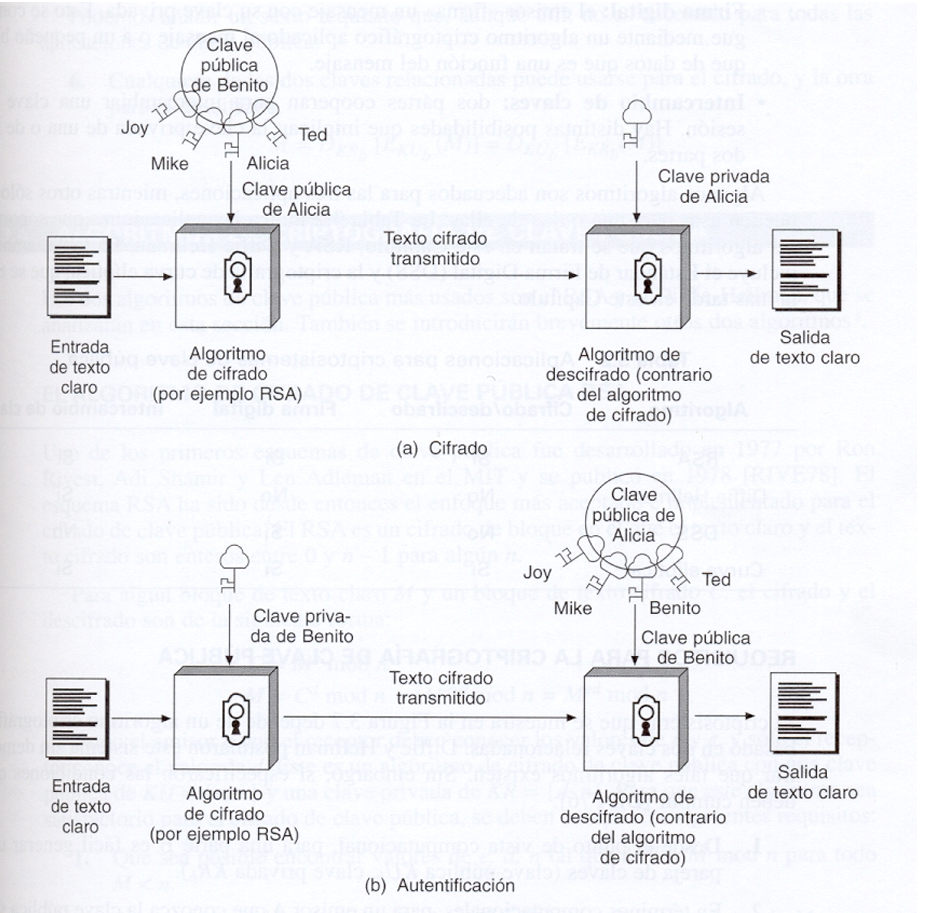
\includegraphics[width=0.7\textwidth]{./Graphics/cifrado_esquema.png}
    \caption{\scriptsize Esquema de uso de los algoritmos de cifrado asimétrico.}
    \label{fig:Cipher}
\end{figure}

Pasos esenciales del cifrado de clave pública
\begin{itemize}
  \item \textbf{Generación de llaves}: Cada usuario genera un par de llaves para cifrar y descifrar mensajes.
  \item \textbf{Distribución de la llave pública}: Cada usuario coloca una de las llaves (la pública) en un registro accesible. La llave privada se mantiene secreta.
  \item \textbf{Proceso de cifrado}:
  \begin{itemize}
    \item Si Bob desea enviar un mensaje confidencial a Alice, utiliza la llave pública de Alice para cifrarlo.
    \item Al recibir el mensaje, Alice lo descifra utilizando su llave privada.
  \end{itemize}  
  \item \textbf{Confidencialidad asegurada}:
  \begin{itemize}
    \item Todos los participantes tienen acceso a las llaves públicas de otros usuarios.
    \item Las llaves privadas nunca necesitan ser compartidas.
    \item Mientras una llave privada esté protegida, la comunicación permanece segura.
  \end{itemize}  
  \item \textbf{Rotación de llaves}: En caso de ser necesario, cualquier usuario puede generar una nueva llave privada y publicar la nueva llave pública para reemplazar la anterior.
\end{itemize}  
Este enfoque asegura:
\begin{itemize}
  \item Confidencialidad: Solo el receptor (Alice) puede descifrar el mensaje.
  \item Gestión sencilla de llaves: No es necesario compartir o enviar la llave privada, reduciendo el riesgo de compromiso.
\end{itemize}

Un criptosistema con estas características no es suficientemente seguro, ya que sigue siendo vulnerable a ataques de tipo \textit{\textbf{Man-in-the-Middle}} (como se muestra en la figura \ref{fig:MIM}) y a la suplantación de identidad. Por ejemplo, si un usuario \textbf{D} publica su clave pública \textbf{PUd} haciéndola pasar por la clave de otro usuario \textbf{B}, cualquier persona que intente comunicarse con \textbf{B} podría utilizar \textbf{PUd} para cifrar su mensaje, creyendo erróneamente que está enviándolo de forma segura a \textbf{B}. En este caso, si \textbf{D} intercepta el mensaje, podrá descifrarlo fácilmente con su clave privada, comprometiendo así la confidencialidad de la comunicación.

\begin{figure}[!htbp]
    \centering
    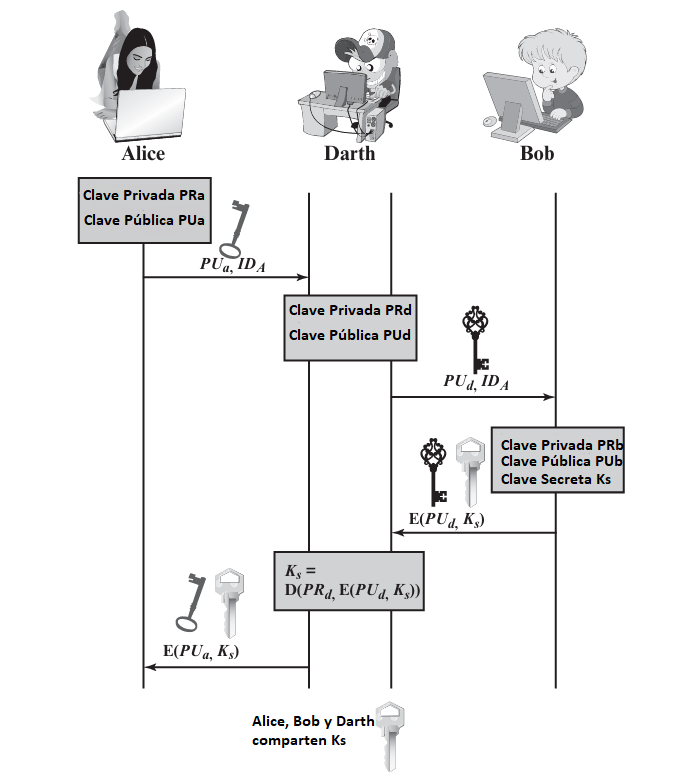
\includegraphics[width=0.7\textwidth]{./Graphics/MIM.png}
    \caption{\scriptsize Ataque \textit{Man-in-the-Middle}.}
    \label{fig:MIM}
\end{figure}

Para mitigar riesgos de seguridad como los mencionados, se emplean los \textbf{certificados digitales}, que actúan como una prueba firmada que garantiza que una identidad es realmente quien dice ser. 
La emisión de estos certificados recae en una autoridad de confianza conocida como \textbf{CA} (por sus siglas en inglés, \textit{Certification Authority}). 
Esta autoridad debe contar con su propio certificado que la valide como una \textbf{CA} confiable, emitido por otra \textbf{CA} o, en última instancia, por una autoridad raíz. 
Toda esta información debe estar reflejada en el certificado, creando así una red de confianza transparente y auditable.

\section{Infraestructura de Clave Pública}

La infraestructura de clave pública, como se mencionó anteriormente, es el conjunto de entidades que incluyen software, políticas, procedimientos, hardware y personas, que participan en la gestión de la emisión, verificación y revocación de certificados digitales. Su principal objetivo es permitir la adquisición de claves públicas de manera segura, conveniente y eficiente.

\subsection{Componentes principales de una PKI}

Una \textbf{PKI} se compone de varios elementos fundamentales, descritos a continuación:

\begin{itemize}
    \item \textbf{Entidad final (End Entity)}: Término genérico para designar a los usuarios finales, dispositivos (por ejemplo, servidores, enrutadores) u otras entidades que pueden ser identificadas en el campo de sujeto de un certificado de clave pública. Las entidades finales suelen consumir y/o soportar servicios relacionados con la PKI.
    
    \item \textbf{Autoridad de certificación (CA)}: Es la emisora de certificados y, en la mayoría de los casos, de listas de revocación de certificados (\textbf{CRLs}). También puede encargarse de diversas funciones administrativas, aunque a menudo estas se delegan a una o más Autoridades de Registro (\textbf{RA}).
    
    \item \textbf{Autoridad de registro (RA)}: Componente opcional que puede asumir varias funciones administrativas delegadas por la CA. Por lo general, la RA está asociada con el proceso de registro de entidades finales, pero también puede asistir en otras áreas.
    
    \item \textbf{Emisor de CRL (CRL Issuer)}: Componente opcional al que una CA puede delegar la publicación de listas de revocación de certificados (\textbf{CRLs}).
    
    \item \textbf{Repositorio (Repository)}: Término genérico que se refiere a cualquier método para almacenar certificados y listas de revocación, de manera que puedan ser recuperados por las entidades finales.
\end{itemize}

\subsection{Funcionalidades clave de una PKI}

Una PKI debe ser capaz de cumplir con las siguientes funcionalidades esenciales:
\begin{itemize}
    \item \textbf{Registro:} Es el proceso inicial donde un usuario se identifica ante una CA o RA, iniciando la inscripción en la PKI.
    \item \textbf{Inicialización:} Configuración inicial de los materiales criptográficos necesarios para la operación segura del sistema cliente.
    \item \textbf{Certificación:} Emisión de un certificado que vincula una clave pública con una identidad.
    \item \textbf{Recuperación de pares de claves:} Mecanismo para recuperar claves de desencriptación en caso de pérdida de acceso.
    \item \textbf{Actualización de pares de claves:} Renovación periódica de claves y certificados asociados.
    \item \textbf{Solicitud de revocación:} Proceso para revocar certificados en caso de compromisos o cambios relevantes.
    \item \textbf{Certificación cruzada:} Establecimiento de confianza mutua entre dos CA mediante certificados cruzados.
\end{itemize}

\subsubsection{Estándares Relevantes en PKI}

Dentro de la PKI, existen estándares y protocolos ampliamente aceptados que garantizan la interoperabilidad y seguridad de las operaciones. Entre los más destacados se encuentran:

\paragraph{X.509}  
El estándar \textbf{X.509} \cite{rfc5280}, desarrollado por la \textit{International Telecommunication Union - Telecommunication Standardization Sector (ITU-T)}, define el formato de los certificados digitales y las listas de revocación de certificados (CRL). Este estándar establece la estructura básica para las PKI modernas, permitiendo la creación de una jerarquía de confianza mediante certificados emitidos por Autoridades Certificadoras (CA).

\begin{itemize}
    \item Los certificados X.509 incluyen información como el nombre del sujeto, el emisor, el período de validez y la clave pública asociada.
    \item Se utilizan firmas digitales para garantizar la autenticidad e integridad de los certificados.
    \item La versión 3 de X.509 permite el uso de extensiones para adaptarse a requerimientos específicos, como políticas de certificados o restricciones de uso de claves.
\end{itemize}

\paragraph{TLS (Transport Layer Security)}  
El protocolo \textbf{TLS} garantiza comunicaciones seguras en redes, y utiliza certificados X.509 para autenticar las partes involucradas y negociar claves de cifrado \cite{dierks2008tls}. TLS es esencial en aplicaciones como HTTPS, correo electrónico seguro y comunicaciones en tiempo real.

\begin{itemize}
    \item \textbf{Autenticación mutua}: Los certificados permiten autenticar tanto al servidor como al cliente.
    \item \textbf{Cifrado de datos}: Utiliza algoritmos modernos, como AES, para proteger la confidencialidad de la información.
    \item \textbf{Negociación segura de claves}: Emplea mecanismos como \textit{Diffie-Hellman} o \textit{Elliptic Curve Diffie-Hellman} (ECDH).
\end{itemize}

\paragraph{Otros Estándares Relevantes}
Además de X.509 y TLS, existen otros estándares y protocolos importantes que complementan las funcionalidades de la PKI:

\begin{itemize}
    \item \textbf{OCSP (Online Certificate Status Protocol)}: Permite verificar en tiempo real el estado de un certificado digital, reemplazando o complementando las listas de revocación (CRL) \cite{rfc2560}.
    \item \textbf{S/MIME (Secure/Multipurpose Internet Mail Extensions)}: Garantiza la confidencialidad e integridad de los correos electrónicos mediante PKI.
    \item \textbf{IPSec (Internet Protocol Security)}: Asegura las comunicaciones IP mediante autenticación y cifrado, utilizando certificados X.509 para la autenticación \cite{kent1998ipsec}.
    \item \textbf{CMP (Certificate Management Protocol)}: Facilita la gestión automatizada de certificados, incluyendo emisión, renovación y revocación.
\end{itemize}

\section{Blockchain}

La \textit{blockchain} es una tecnología de registro distribuido que permite mantener un historial inmutable y transparente de transacciones. Este epígrafe incluirá:

\begin{itemize}
    \item Concepto, definición e historia de \textit{\textbf{blockchain}}.
    \item Principales características: descentralización, inmutabilidad, seguridad y transparencia.
    \item Componentes clave: bloques, nodos, algoritmos de consenso.
    \item Usos y aplicaciones principales.
\end{itemize}

\subsection{Historia de Blockchain}

El concepto de \textit{blockchain}, o cadena de bloques, tiene sus raíces en un artículo seminal titulado ``Bitcoin: A Peer-to-Peer Electronic Cash System'', publicado en 2008 por una persona o grupo bajo el seudónimo de \textbf{Satoshi Nakamoto} \cite{nakamoto2008bitcoin}. Aunque blockchain es ampliamente conocida por ser la tecnología subyacente detrás del \textit{Bitcoin}, su origen conceptual puede rastrearse décadas atrás.

En 1991, los investigadores \textbf{Stuart Haber} y \textbf{W. Scott Stornetta} introdujeron por primera vez la idea de una estructura encadenada de bloques para proteger la integridad de documentos digitales mediante marcas de tiempo \cite{haber1991timestamping}. Este esquema aseguraba que los documentos no pudieran ser alterados sin invalidar los registros posteriores, lo que sentó las bases para lo que hoy conocemos como blockchain.

Más adelante, en 1998, \textbf{Nick Szabo} propuso un sistema llamado \textit{Bit Gold}, que utilizaba un mecanismo descentralizado para crear un bien digital escaso mediante pruebas de trabajo (Proof-of-Work, PoW). Aunque \textit{Bit Gold} nunca fue implementado, se considera un precursor conceptual del \textit{Bitcoin} \cite{szabo1998bitgold}.

El verdadero avance llegó en 2009 con la creación de \textit{Bitcoin}, la primera implementación práctica de blockchain. Este sistema no solo ofreció una nueva forma de moneda digital descentralizada, sino que introdujo un mecanismo innovador para garantizar la confianza entre participantes anónimos mediante la combinación de pruebas de trabajo, criptografía asimétrica y un modelo de consenso descentralizado \cite{nakamoto2008bitcoin}.

Con el tiempo, la tecnología blockchain ha evolucionado más allá de las criptomonedas, encontrando aplicaciones en áreas como contratos inteligentes, cadenas de suministro, identidad digital y más. En 2015, la aparición de \textit{Ethereum}, una plataforma que extendió la funcionalidad de blockchain al permitir la ejecución de contratos inteligentes, marcó otro hito importante en la historia de esta tecnología.

Hoy en día, blockchain se percibe como una herramienta clave para garantizar transparencia, seguridad y descentralización en múltiples dominios, convirtiéndose en una piedra angular de la infraestructura tecnológica moderna.

\subsection{Principales Características de Blockchain}

Las blockchains destacan por su capacidad para ofrecer soluciones innovadoras en el ámbito del almacenamiento y transferencia de información gracias a características únicas. A continuación, se describen las más relevantes: \textbf{descentralización}, \textbf{inmutabilidad}, \textbf{seguridad} y \textbf{transparencia}.

\subsubsection{Descentralización}  
La descentralización es una de las propiedades más importantes de blockchain, eliminando la necesidad de intermediarios para el manejo y verificación de datos. En lugar de depender de una autoridad central, la red está compuesta por nodos distribuidos que mantienen una copia sincronizada del registro completo. 

\begin{itemize}
    \item \textbf{Red distribuida}: Cada nodo en la red posee una copia del libro mayor, lo que asegura redundancia y evita puntos únicos de falla.
    \item \textbf{Autonomía}: La validación de transacciones se realiza a través de mecanismos de consenso como \textit{Proof of Work} (PoW), \textit{Proof of Stake} (PoS) u otros, reduciendo la dependencia de terceras partes.
    \item \textbf{Resiliencia}: Al no depender de un servidor central, las blockchains son altamente resistentes a ataques como \textit{Distributed Denial of Service} (DDoS) y otros que buscan interrumpir su operación.
\end{itemize}

\subsubsection{Inmutabilidad}  
La inmutabilidad asegura que, una vez registrada, la información dentro de la blockchain, resulte extremadamente complejo modificar o eliminar la misma. Esta característica se logra mediante el uso de criptografía y la estructura de bloques encadenados.

\begin{itemize}
    \item \textbf{Registro permanente}: Cada bloque contiene un identificador único (hash) basado en su contenido y en el hash del bloque anterior, formando una cadena que dificulta cualquier alteración.
    \item \textbf{Protección contra manipulaciones}: Si un atacante intenta modificar un bloque, necesitaría rehacer todos los bloques subsiguientes, lo que sería computacionalmente inviable en redes grandes y bien distribuidas.
    \item \textbf{Integridad}: Esta propiedad garantiza que los datos almacenados en la blockchain permanecen consistentes y verificables con el tiempo.
\end{itemize}

\subsubsection{Seguridad}  
La seguridad en blockchain es uno de sus pilares fundamentales, basado en el uso de algoritmos criptográficos avanzados y su arquitectura distribuida. 

\begin{itemize}
    \item \textbf{Criptografía}: Las transacciones están protegidas mediante algoritmos como ECDSA, y los hashes se generan con funciones como SHA-256.
    \item \textbf{Autenticación y privacidad}: Las claves públicas y privadas permiten autenticar usuarios y garantizar la privacidad de los datos. Solo quien posea la clave privada puede autorizar transacciones.
    \item \textbf{Resistencia a ataques}: Su diseño distribuido hace que sea extremadamente difícil comprometer la red en su totalidad, ya que un atacante necesitaría controlar la mayoría de los nodos para realizar un ataque del tipo \textit{51\%}.
\end{itemize}

\subsubsection{Transparencia}  
La transparencia en blockchain se refiere a que todas las transacciones registradas en la red son accesibles y verificables por cualquier participante, aunque se preserve la privacidad de los usuarios.

\begin{itemize}
    \item \textbf{Libro mayor público}: En blockchains públicas como Bitcoin y Ethereum, cualquier persona puede examinar todas las transacciones realizadas desde la creación de la red.
    \item \textbf{Auditabilidad}: La naturaleza transparente de la blockchain permite auditorías completas y verificaciones independientes en cualquier momento.
    \item \textbf{Equilibrio entre privacidad y visibilidad}: Aunque las transacciones son visibles, los usuarios permanecen anónimos al usar direcciones públicas que no revelan identidades reales.
\end{itemize}

\subsection{Componentes clave}

La tecnología blockchain se compone de varios elementos esenciales que trabajan juntos para garantizar su funcionamiento seguro, transparente y descentralizado. Los tres componentes clave son los \textbf{bloques}, los \textbf{nodos} y los \textbf{algoritmos de consenso}. A continuación, se detalla el funcionamiento de cada uno de estos componentes.

\subsubsection{Bloques en Blockchain}

Un \textbf{bloque} en una blockchain es una unidad de almacenamiento que contiene un conjunto de transacciones o datos. En términos simples, un bloque puede considerarse como una "página"\ \ de un libro de registros, y cada nuevo bloque es una "página" que se añade secuencialmente al libro.

\textbf{Componentes de un Bloque}:
\begin{itemize}
    \item \textbf{Encabezado del bloque (Block Header)}: Contiene metadatos esenciales sobre el bloque, como:
    \begin{itemize}
        \item \textit{Hash del bloque anterior}: Enlaza este bloque al bloque anterior en la cadena, creando una secuencia inmutable.
        \item \textit{Timestamp (marca temporal)}: La hora exacta en que se creó el bloque.
        \item \textit{Hash del bloque}: Un valor único generado por una función hash que representa el contenido del bloque.
        \item \textit{Merkle Root}: Es un hash que representa todas las transacciones dentro del bloque de manera compacta y eficiente.
        \item \textit{Nonce} (en el caso de Proof of Work): Un número utilizado para facilitar la resolución del problema de la minería.
        \item \textit{Número de bloque}: Identificador único del bloque dentro de la cadena.
    \end{itemize}
    \item \textbf{Cuerpo del bloque (Block Body)}: Contiene las transacciones, que son los datos reales que se están registrando en la blockchain. Estas transacciones pueden ser cualquier tipo de información, dependiendo de la blockchain (por ejemplo, transacciones financieras en Bitcoin o contratos inteligentes en Ethereum).
\end{itemize}

\textbf{Función de los Bloques}:
\begin{itemize}
    \item \textit{Inmutabilidad}: Una vez que un bloque se añade a la cadena, se vuelve muy difícil de alterar debido a los hashes y la interdependencia entre bloques.
    \item \textit{Transparencia}: Todos los participantes de la red pueden verificar el contenido de los bloques.
    \item \textit{Seguridad}: Debido al algoritmo de hash y la interconexión de los bloques, es extremadamente difícil modificar un bloque sin que se detecte.
\end{itemize}

\subsubsection{Nodos en Blockchain}

Un \textbf{nodo} es cualquier dispositivo o entidad que participa en la red blockchain. Los nodos mantienen la base de datos distribuida y realizan diversas funciones según su tipo.

\textbf{Tipos de Nodos}:
\begin{itemize}
    \item \textbf{Nodos completos (Full Nodes)}: Estos nodos almacenan toda la blockchain, incluyendo todos los bloques desde el génesis (primer bloque) hasta el último. Verifican todas las transacciones y bloques, y son fundamentales para la seguridad y la descentralización de la red. Pueden validar transacciones y bloques.
    \item \textbf{Nodos ligeros (Light Nodes)}: Solo almacenan una parte de la blockchain, generalmente los encabezados de los bloques, y dependen de los nodos completos para obtener información más detallada. Son útiles cuando se requiere un uso de recursos reducido, pero con la limitación de no realizar validaciones completas.
    \item \textbf{Nodos de minería (Mining Nodes)}: Estos nodos realizan la labor de minería en cadenas como Bitcoin. Resuelven problemas computacionales complejos para encontrar un bloque válido, lo cual es parte del algoritmo de consenso (por ejemplo, \textit{Proof of Work}). Este tipo de nodo también es un \textbf{nodo completo}, ya que necesita almacenar toda la blockchain.
    \item \textbf{Nodos de consenso}: Estos nodos participan en el proceso de consenso de la blockchain, es decir, ayudan a asegurar que todos los participantes de la red estén de acuerdo con el estado de la blockchain y validan las transacciones.
\end{itemize}

\textbf{Función de los Nodos}:
\begin{itemize}
    \item \textit{Verificación de Transacciones}: Los nodos validan las transacciones antes de que se incluyan en un bloque.
    \item \textit{Distribución de Información}: Los nodos son responsables de propagar los bloques y transacciones a través de la red, asegurando que todos los participantes tengan la misma información.
    \item \textit{Seguridad}: Como la blockchain es descentralizada, los nodos colaboran para mantener la integridad de la red. Cuantos más nodos haya, más difícil será atacar la red.
\end{itemize}

\subsubsection{Algoritmos de Consenso en Blockchain}

El \textbf{algoritmo de consenso} es el mecanismo que permite que todos los nodos de una red blockchain estén de acuerdo sobre el estado actual de la cadena de bloques. Como no hay una autoridad central en una blockchain, el consenso asegura que todos los participantes puedan llegar a un acuerdo sobre qué transacciones son válidas.

\textbf{Tipos de Algoritmos de Consenso}:
\begin{itemize}
    \item \textbf{Proof of Work (PoW)}:
    \begin{itemize}
        \item Usado por \textit{Bitcoin} y otras criptomonedas.
        \item En este algoritmo, los nodos (mineros) deben resolver problemas matemáticos complejos para encontrar un bloque válido. Este proceso consume mucho poder de cómputo y energía.
        \item El primer nodo que resuelve el problema recibe una recompensa (minería) y el bloque se agrega a la blockchain.
        \item \textit{Seguridad}: Debido a que un atacante tendría que dominar más del 50\% del poder computacional de la red para alterar un bloque, PoW es muy seguro pero ineficiente en términos de consumo energético.
        \begin{figure}[!htbp]
            \centering
            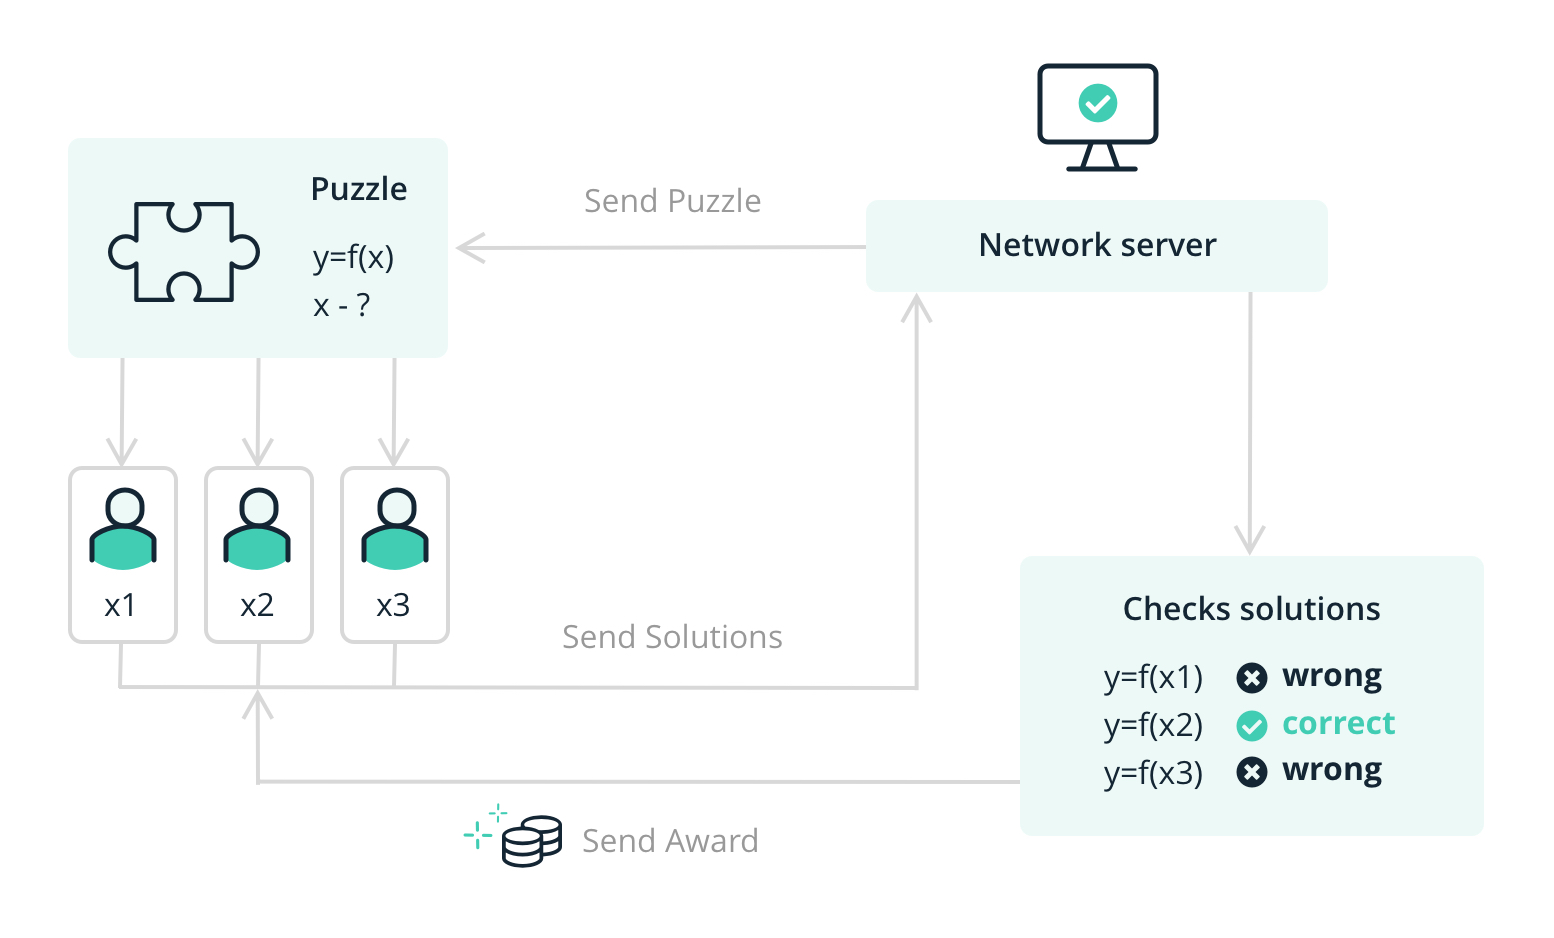
\includegraphics[width=0.7\textwidth]{./Graphics/PoW.png}
            \caption{\textit{PoW}.}
            \label{fig:PoW}
        \end{figure}
    \end{itemize}
    
\

\

    \item \textbf{Proof of Stake (PoS)}:
    \begin{itemize}
        \item Utilizado por \textit{Ethereum 2.0} y otras criptomonedas.
        \item En este modelo, los validadores son seleccionados para crear un nuevo bloque en función de la cantidad de criptomoneda que tienen en "stake" (bloqueada) como garantía. Los validadores reciben recompensas por validar bloques correctamente.
        \item \textit{Eficiencia}: PoS es más eficiente que PoW porque no requiere tanta potencia de cómputo.
        \item \textit{Seguridad}: En teoría, un atacante necesitaría controlar más del 50\% del "stake" total para comprometer la red.
        \begin{figure}[!htbp]
            \centering
            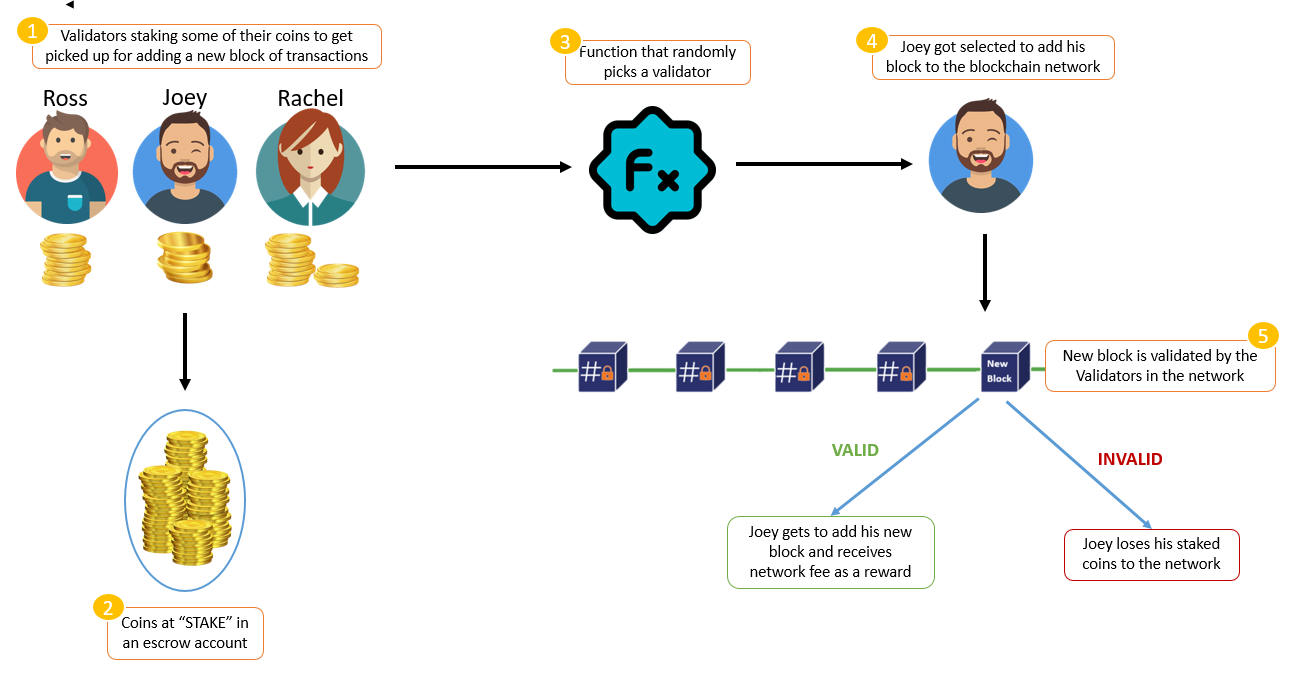
\includegraphics[width=0.7\textwidth]{./Graphics/PoS.png}
            \caption{\textit{PoS}.}
            \label{fig:PoS}
        \end{figure} 
    \end{itemize}

\

\

    \item \textbf{Delegated Proof of Stake (DPoS)}:
    \begin{itemize}
        \item Usado por \textit{EOSIO} \cite{eosio} y otras redes.
        \item Es una versión de PoS donde los participantes votan por representantes (delegados) que validan las transacciones en su nombre. Esto mejora la escalabilidad y eficiencia, pero puede centralizar el poder de validación.
        \begin{figure}[!htbp]
            \centering
            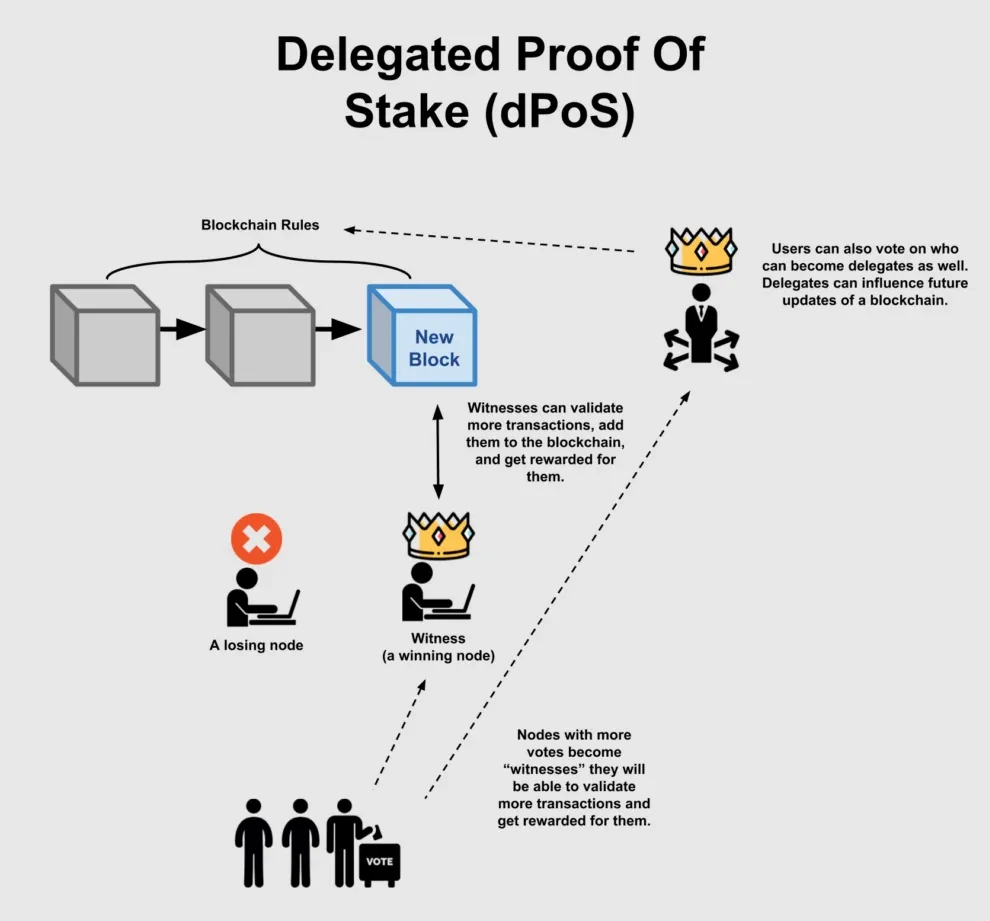
\includegraphics[width=0.5\textwidth]{./Graphics/dPoS.png}
            \caption{\textit{dPoS}.}
            \label{fig:dPoS}
        \end{figure}
    \end{itemize}

\

\

    \item \textbf{Proof of Authority (PoA)}:
    \begin{itemize}
        \item En este sistema, los nodos de validación están predefinidos y son conocidos. Estos nodos son seleccionados con base en su reputación y autoridad.
        \item Usado en redes privadas o de consorcio, donde la confianza en los validadores es clave.
        \begin{figure}[!htbp]
            \centering
            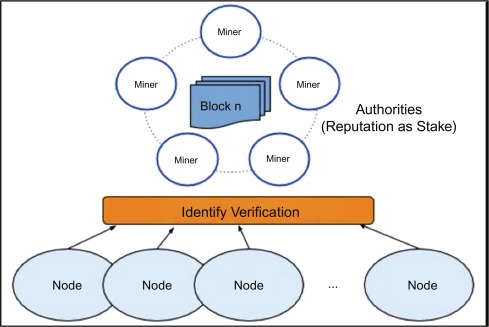
\includegraphics[width=0.7\textwidth]{./Graphics/PoA.png}
            \caption{\textit{PoA}.}
            \label{fig:Po}
        \end{figure}
    \end{itemize}

\end{itemize}

\subsection{Usos y Aplicaciones de Blockchain}

\begin{itemize}
    \item \textbf{Criptomonedas:} Blockchain se usa en Bitcoin, Ethereum y otras criptomonedas para permitir intercambios de valor descentralizados, eliminando intermediarios como los bancos y asegurando transacciones rápidas y económicas.
    
    \item \textbf{Contratos Inteligentes (Smart Contracts):} Programas autoejecutables que se ejecutan cuando se cumplen condiciones predefinidas. Automatización de contratos en bienes raíces, seguros, préstamos, etc.
    
    \item \textbf{Gestión de la Cadena de Suministro:} Rastreabilidad y transparencia de productos a lo largo de la cadena de suministro. Aplicaciones en alimentos, medicamentos y productos de lujo para prevenir fraudes.
        
    \item \textbf{Gobernanza Descentralizada:} Creación de sistemas de gobernanza más transparentes y participativos en organizaciones descentralizadas y autónomas (DAO). Se utiliza en votaciones electrónicas y decisiones colectivas.
    
    \item \textbf{Finanzas Descentralizadas (DeFi):} Plataformas financieras sin intermediarios, como préstamos, seguros, intercambio de activos y DEX. Promueve el ahorro y préstamo en un entorno descentralizado.
    
    \item \textbf{Propiedad Intelectual y Derechos de Autor:} Blockchain gestiona los derechos de autor y permite la tokenización de activos digitales como música, arte y coleccionables (NFTs), garantizando una compensación justa a los creadores.
    
    \item \textbf{Sector Salud:} Blockchain mejora la gestión de registros médicos electrónicos y rastrea la cadena de suministro de medicamentos, evitando falsificaciones y mejorando la calidad del servicio.
    
    \item \textbf{Energía y Sostenibilidad:} Facilita redes de energía descentralizadas donde los usuarios venden y compran energía renovable. También permite el rastreo de huella de carbono en empresas y gobiernos.
    
    \item \textbf{Votación Electrónica:} Proporciona un sistema de votación seguro, transparente y verificable, garantizando la integridad de los votos y previniendo fraudes electorales.
    
    \item \textbf{Tokenización de Activos:} Transformación de activos físicos o digitales en tokens que se pueden negociar, aplicable a inmuebles, activos financieros y productos de lujo.
    
    \item \textbf{Redes Sociales Descentralizadas:} Plataformas donde los usuarios mantienen el control sobre sus datos y contenido, protegiendo la privacidad y eliminando intermediarios.
\end{itemize}

\section{Hyperledger Fabric}
\subsubsection{Canales y Nodos en Hyperledger Fabric}

A diferencia de otras blockchains públicas donde todas las transacciones son visibles para todos los participantes, Hyperledger Fabric introduce el concepto de \textbf{canales}\cite{hyperledgerfabric}.

\begin{itemize}
    \item Un \textbf{canal} es una subred dentro de la blockchain donde un conjunto específico de participantes puede comunicarse de manera privada.
    \item Cada canal es gestionado por nodos llamados \textbf{Orderers}, los cuales tienen la función de organizar las transacciones en bloques y distribuirlos a los nodos validadores (peers).
    \item Los canales pueden ser configurados para que solo ciertas organizaciones tengan acceso a los datos y transacciones dentro de ellos.
\end{itemize}

\subsubsection{Estructura de Organizaciones y Peers}

Hyperledger Fabric permite la participación de múltiples \textbf{organizaciones}\cite{hyperledgerfabric}, cada una con su propio conjunto de nodos llamados \textbf{Peers}.

\begin{itemize}
    \item \textbf{Peers:} Son los nodos que mantienen la información del ledger y ejecutan los contratos inteligentes (chaincodes).
    \item \textbf{Organizaciones:} Son entidades dentro de la red que administran sus propios peers y participan en la toma de decisiones sobre la gestión del canal.
    \item \textbf{Endorsing Peers:} Son aquellos que validan y ejecutan transacciones antes de que sean enviadas a los orderers para su inclusión en un bloque.
    \item \textbf{Anchor Peer:} Son nodos dentro de una organización que facilita la comunicación entre distintas organizaciones en un canal. Sirve como punto de referencia para compartir información sobre la topología de la red y permite que los peers de diferentes organizaciones se descubran entre sí sin necesidad de conexión directa.
\end{itemize}


\begin{figure}[!htbp]
    \centering
    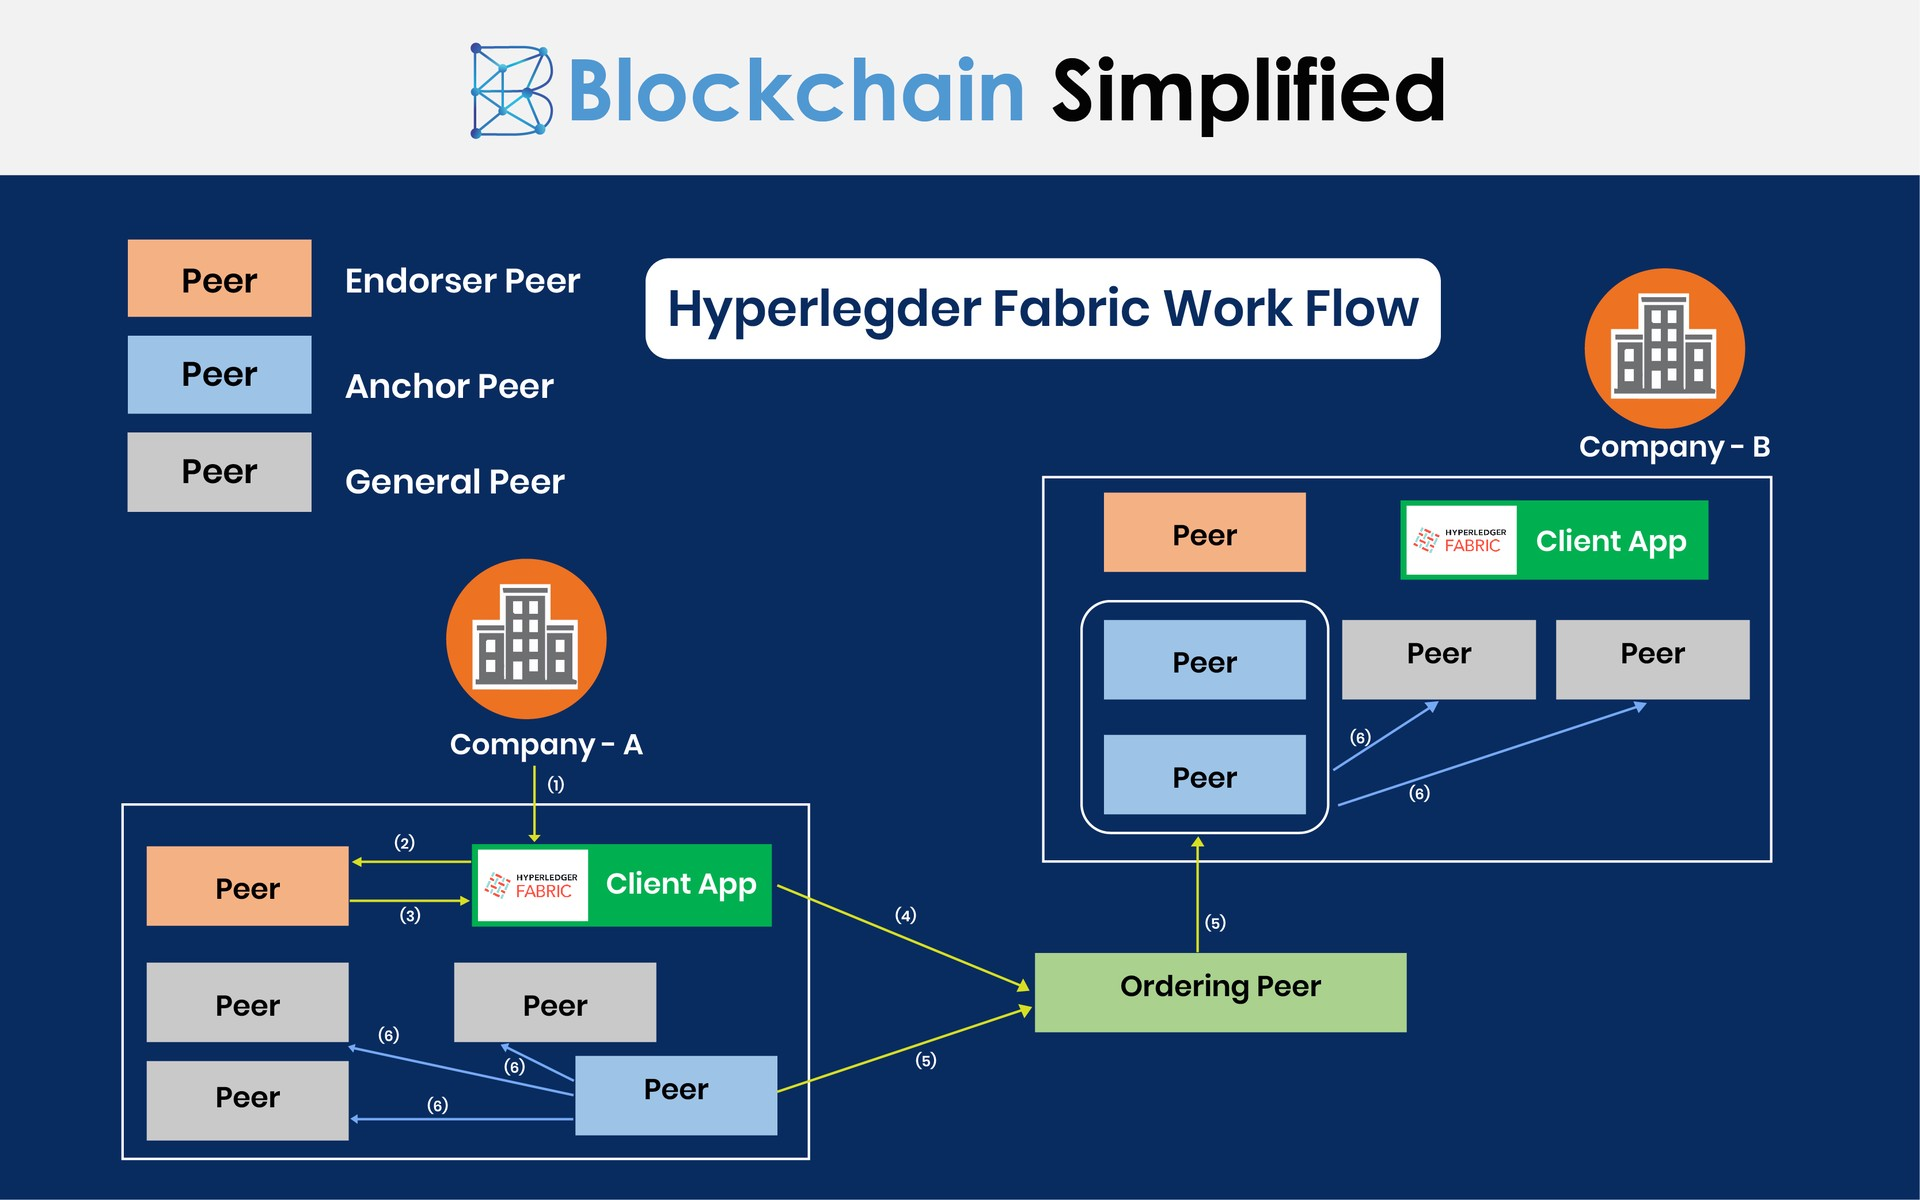
\includegraphics[width=0.7\textwidth]{./Graphics/HLF.png}
    \caption{\textit{Hyperledger Fabric}.}
    \label{fig:HLF}
\end{figure}
\chapter{Estado del Arte}

Este capítulo explora diversas propuestas que integran blockchain en la PKI, analizando sus ventajas, desafíos y aplicaciones prácticas. Se examinarán modelos como CertLedger, que utiliza blockchain para mejorar la transparencia y seguridad en la gestión de certificados digitales, y otras arquitecturas que buscan superar las limitaciones de las PKI tradicionales mediante enfoques descentralizados y dinámicos. A través de este análisis, se pretende proporcionar una visión comprensiva del estado actual de la tecnología y su potencial para revolucionar la gestión de identidades digitales en diversos.

\section{CertLedger: Un Nuevo Modelo de PKI con Transparencia de Certificados Basado en Blockchain}

En 2018, Kubilay, Kiraz y Mantar introdujeron CertLedger \cite{Kubilay2018}, una arquitectura de PKI que utiliza blockchain para mejorar la transparencia y seguridad en la gestión de certificados digitales. A diferencia de las PKI tradicionales, donde las Autoridades Certificadoras (CA) son entidades centralizadas y de confianza, CertLedger propone registrar todos los eventos relacionados con certificados, como emisión, renovación y revocación, en una blockchain pública. Este enfoque busca eliminar ataques como el ``split-world'' y reducir la dependencia de las CA tradicionales.

\textbf{Ventajas:}

\begin{itemize}
  \item \textbf{Transparencia y Trazabilidad:} Al registrar todas las operaciones en una blockchain pública, se garantiza una trazabilidad completa de los certificados, facilitando auditorías y aumentando la confianza en el sistema.
  \item \textbf{Eliminación de Intermediarios:} Al centralizar la gestión de certificados en la blockchain, se reduce la necesidad de intermediarios, disminuyendo costos y simplificando la infraestructura.
  \item \textbf{Revocación Eficiente:} La revocación de certificados comprometidos se gestiona de manera rápida y confiable, asegurando que los nodos no validen información desactualizada o fraudulenta.
\end{itemize}

\textbf{Desventajas:}

\begin{itemize}
  \item \textbf{Escalabilidad:} Las soluciones basadas en blockchain pueden enfrentar dificultades para manejar grandes volúmenes de transacciones en tiempo real, lo que podría afectar su rendimiento en entornos de alta demanda.
  \item \textbf{Adopción Empresarial:} La implementación de este modelo en entornos corporativos puede ser desafiante debido a la necesidad de interoperabilidad con sistemas existentes y posibles resistencias al cambio.
\end{itemize}

\section{PKI Dinámica Descentralizada Basada en Blockchain}

Toorani y Gehrmann, en 2020, propusieron un modelo de PKI dinámico que combina blockchain con el concepto de "web of trust" \cite{Toorani2020}. Este enfoque busca superar las limitaciones de las PKI tradicionales al permitir la validación de certificados entre usuarios sin depender de autoridades centralizadas. En su propuesta, blockchain actúa como un registro descentralizado e inmutable para los certificados digitales, proporcionando transparencia y resistencia a ataques. El modelo adopta la "web of trust", donde los usuarios pueden validar y firmar mutuamente sus certificados, distribuyendo la confianza de manera dinámica. Además, es un sistema adaptable que permite agregar nuevos participantes y revocar certificados sin necesidad de reconstruir toda la infraestructura.

\textbf{Ventajas:}

\begin{itemize}
  \item \textbf{Descentralización:} Elimina la dependencia de una autoridad certificadora única, reforzando la seguridad y reduciendo puntos únicos de fallo.
  \item \textbf{Escalabilidad:} Permite la incorporación de nuevos participantes en la red sin necesidad de reestructurar la infraestructura existente.
  \item \textbf{Transparencia:} Todas las transacciones relacionadas con los certificados se registran en la blockchain, facilitando auditorías y aumentando la confianza en el sistema.
  \item \textbf{Adaptabilidad:} El sistema se ajusta a diferentes necesidades y contextos, permitiendo una gestión flexible de certificados.
\end{itemize}

\textbf{Desventajas:}

\begin{itemize}
  \item \textbf{Complejidad Operativa:} En redes grandes, la gestión de la confianza distribuida puede ser compleja y requerir una coordinación significativa entre los participantes.
  \item \textbf{Infraestructura Requerida:} La implementación requiere una infraestructura blockchain robusta, lo que puede ser costoso y técnicamente desafiante.
  \item \textbf{Desempeño:} El sistema puede ser más lento que una PKI centralizada debido a las limitaciones inherentes de la tecnología blockchain.
  \item \textbf{Establecimiento de Confianza Inicial:} Establecer relaciones de confianza en redes completamente nuevas puede ser un reto significativo.
\end{itemize}
\section{PKI Basada en Blockchain dentro de una Organización Corporativa: Ventajas y Desafíos}

En 2024, Springer y Haindl analizaron cómo la tecnología blockchain puede integrarse en una PKI dentro de una organización corporativa, comparándola con los sistemas PKI tradicionales \cite{Springer2024}. Los principales enfoques del estudio incluyen la descentralización de la confianza, la inmutabilidad y la transparencia de los certificados, la auditoría mejorada y la reducción de costos operativos.

\textbf{Ventajas:}

\begin{itemize}
  \item \textbf{Descentralización de la Confianza:} Blockchain permite distribuir la confianza entre varios nodos, eliminando la necesidad de una autoridad central y mejorando la resiliencia del sistema ante posibles ataques.
  \item \textbf{Inmutabilidad y Transparencia:} Blockchain asegura que los registros de certificados no puedan ser alterados una vez emitidos, garantizando su integridad. Además, la transparencia de blockchain permite auditar continuamente todas las transacciones, facilitando la detección y resolución de problemas relacionados con los certificados.
  \item \textbf{Reducción de Costos Operativos:} La adopción de blockchain puede reducir los costos operativos al eliminar la necesidad de intermediarios y simplificar los procesos manuales en la gestión de certificados.
\end{itemize}

\textbf{Desventajas:}

\begin{itemize}
  \item \textbf{Complejidad de Implementación:} Integrar una PKI basada en blockchain en una organización puede requerir una reestructuración significativa de la infraestructura existente, lo que implica desafíos técnicos y operativos.
  \item \textbf{Cumplimiento Normativo:} El cumplimiento de normativas regulatorias y legales representa un desafío adicional, ya que las organizaciones deben asegurarse de que la implementación de la blockchain cumpla con las leyes y regulaciones vigentes.
  \item \textbf{Escalabilidad:} Las soluciones basadas en blockchain pueden enfrentar dificultades para manejar grandes volúmenes de transacciones en tiempo real, lo que podría afectar su rendimiento en entornos corporativos de gran escala.
  \item \textbf{Interoperabilidad:} Integrar una PKI basada en blockchain con sistemas y aplicaciones existentes puede ser complejo, requiriendo desarrollos adicionales para asegurar una comunicación fluida entre diferentes plataformas.
  \item \textbf{Resistencia al Cambio:} La adopción de nuevas tecnologías como blockchain puede encontrar resistencia dentro de la organización, especialmente si el personal no está familiarizado con su funcionamiento o beneficios.
\end{itemize}

\section*{Conclusión del Estado del Arte}
Tras analizar los enfoques existentes en la literatura, no se identificaron propuestas que sigan una línea de desarrollo similar a la planteada en este trabajo. La mayoría de las soluciones revisadas se centran en \textit{la descentralización de la PKI mediante el uso de blockchain }, mientras que este estudio propone un enfoque basado en \textit{la incorporación de una PKI tradicional dentro de la arquitectura de Hyperledger Fabric}, permitiendo la autenticación de nodos y la gestión de certificados de manera eficiente dentro de un ecosistema blockchain empresarial.

Dicho enfoque puede traer ventajas como:
\begin{itemize}
  \item \textbf{Aprovechamiento de Infraestructura Existente} – Permite reutilizar una PKI tradicional sin necesidad de rediseñar completamente el sistema de gestión de certificados.
  \item \textbf{Autenticación Eficiente} – Facilita la validación de nodos dentro de Hyperledger Fabric sin depender exclusivamente de su mecanismo nativo de identidad.
  \item \textbf{Cumplimiento Regulatorio} – Mantiene compatibilidad con estándares y normativas PKI, facilitando la adopción en entornos empresariales.
  \item \textbf{Interoperabilidad} – Permite integrar soluciones blockchain con sistemas tradicionales que ya operan con PKI, mejorando la compatibilidad en infraestructuras híbridas.
\end{itemize}

\chapter{Resultados y Discusión}\label{chapter:implementation}

\section{Diseño del modelo}
\begin{itemize}
    \item Diseñar una API que funcione de CA de una PKI 
    \item Configurar una red de Hyperledger Fabric\cite{hyperledgerfabric} capaz de usar los servicios de la PKI antes mencionada para autenticar sus nodos.
\end{itemize}


\section{Implementación de una PKI para la Autenticación de Nodos en Hyperledger Fabric}
La autenticación de los nodos en una red de Hyperledger Fabric\cite{hyperledgerfabric} es un aspecto fundamental para garantizar la seguridad y confianza en las transacciones. Para ello, se diseñó una PKI basada en una API desarrollada en Node.js\cite{nodejs} que actúa como una Autoridad Certificadora (CA). Esta API tiene como función principal gestionar el proceso de emisión de certificados digitales, permitiendo la generación, firma y validación de los mismos. De esta manera, se asegura que cada nodo en la red posea una identidad verificable y protegida contra intentos de suplantación.

\


A continuación se detallará el proceso de implementación de los componentes de la PKI utilizando el framework Express\cite{express} de Node.js para la gestión de servicios REST, Axios\cite{axios} para la comunicación con los clientes y OpenSSL\cite{openssl} como herramienta para la generación de claves, certificados y firmas digitales. Además, se explicará cómo la API desarrollada permite la automatización de la gestión de identidades dentro de la red blockchain.

\subsection{Descripción de la API PKI}

La API desarrollada en Node.js\cite{nodejs} implementa los siguientes servicios principales:

\begin{itemize}
    \item \textbf{Generación y firma de certificados:} La API permite a los nodos solicitar certificados digitales firmados por la CA, asegurando que solo entidades legítimas puedan participar en la red.
    \item \textbf{Validación de certificados:} A través de endpoints específicos, la API verifica la autenticidad de los certificados presentados por los nodos, permitiendo la detección de credenciales falsas o revocadas.
    \item \textbf{Distribución de la CA:} Se proporciona un endpoint que retorna el certificado público de la CA, facilitando su uso para la validación de identidades dentro de la red.
\end{itemize}

\subsection{Generación del Certificado de la CA}

Cuando la API inicia su operación, el primer paso es la generación del certificado raíz de la CA junto con su par de claves criptográficas. Para lograr esto, se utiliza el módulo \texttt{child\_process} de Node.js\cite{nodejs}, que permite ejecutar comandos del sistema. En este caso, se emplea OpenSSL\cite{openssl} para la creación de claves y certificados.

El proceso de generación de la CA sigue los siguientes pasos:

\begin{enumerate}
    \item Se genera una clave privada utilizando el algoritmo ECDSA\cite{ecdsa} con la curva \texttt{prime256v1} (equivalente a P-256). Este algoritmo es requerido por Hyperledger Fabric para la gestión de identidades.
    \item A partir de la clave privada, se genera un certificado autofirmado con una validez predefinida.
    \item La clave privada y el certificado se almacenan en un directorio seguro dentro del servidor.
\end{enumerate}

El comando utilizado en OpenSSL para la generación de la clave privada es:

\

\small{\textbf{openssl ecparam -genkey -name prime256v1 -noout -out ca-key.pem}}

\

Posteriormente, el certificado autofirmado se genera con:

\

\small{\textbf{openssl req -x509 -new -key ca-key.pem -days 365 -out ca-cert.pem -subj "/CN=CA-Hyperledger"}}

\

Este certificado servirá como la base de confianza para la firma de certificados de los nodos en la red.

\subsection{Proceso de Firma de Certificados}

Una vez establecida la CA, se habilita un endpoint en la API denominado \texttt{/sign-csr}, encargado de recibir solicitudes de firma de certificados. El proceso de firma se describe a continuación:

\begin{enumerate}
    \item Un nodo genera una clave privada y un archivo de Solicitud de Firma de Certificado (CSR) en formato PEM.
    \item El nodo envía el CSR al endpoint \texttt{/sign-csr} de la API.
    \item La API verifica la validez del CSR y procede a firmarlo con la clave privada de la CA.
    \item Se devuelve el certificado firmado al nodo solicitante en formato PEM.
\end{enumerate}

Para la firma del CSR, se emplea el siguiente comando de OpenSSL:

\

\small{\textbf{openssl x509 -req -in node-csr.pem -CA ca-cert.pem -CAkey ca-key.pem -CAcreateserial -out node-cert.pem -days 365}}

\

Este proceso garantiza que cada nodo en la red tenga una identidad única y verificable.


La integración de una PKI en Hyperledger Fabric proporciona un mecanismo sólido para la autenticación de nodos dentro de la red blockchain. La implementación de una CA propia mediante una API permite gestionar de manera eficiente la identidad de los participantes, asegurando la confianza y seguridad en las transacciones.

Además, el uso de OpenSSL en combinación con el módulo \texttt{child\_process} de Node.js ha permitido una generación y firma de certificados ágil y automatizada. Esto no solo optimiza el despliegue de la red, sino que también facilita su escalabilidad a futuro.

En general, esta solución mejora significativamente la seguridad y gestión de identidades dentro de Hyperledger Fabric, estableciendo un modelo robusto de autenticación basado en PKI.
\section{Características de Hyperledger Fabric}
Hyperledger Fabric\cite{hyperledgerfabric} es una plataforma de blockchain modular y permisionada diseñada para aplicaciones empresariales. Su arquitectura se basa en una estructura flexible que permite la segmentación de la red en diferentes \textbf{canales}, la gestión descentralizada de organizaciones y la administración de identidades mediante \textbf{Membership Service Providers (MSP)}.


\section{Gestión de Identidades en Hyperledger Fabric}

Para administrar la identidad de los nodos y participantes en la red, Fabric emplea un sistema basado en \textbf{Membership Service Providers (MSP)}\cite{hyperledgerfabric}.

\begin{itemize}
    \item Un \textbf{MSP} es una estructura de carpetas que contiene los certificados y claves criptográficas necesarias para autenticar entidades en la red.
    \item Cada organización debe contar con un MSP para sus nodos, lo que permite la verificación de identidad y la autorización de operaciones dentro del canal.
    \item Fabric proporciona una herramienta llamada \textbf{Fabric CA}, que facilita la creación y gestión de certificados y la estructura MSP.
\end{itemize}

\subsubsection{Generación Manual del MSP}

En caso de no utilizar \textbf{Fabric CA}, el MSP debe ser generado manualmente. Esto implica la creación de claves privadas, certificados de identidad y archivos de configuración que permitan la validación de los participantes en la red. Para ello, se pueden utilizar herramientas como \textbf{OpenSSL}\cite{openssl}, que permite la generación de certificados firmados por una CA personalizada.

\subsection{Motivación para el Uso de Hyperledger Fabric}

Hyperledger Fabric\cite{hyperledgerfabric} se ha convertido en una de las plataformas de blockchain más utilizadas en entornos empresariales debido a su diseño modular, flexibilidad y capacidad para gestionar identidades y permisos de forma granular. A diferencia de otras soluciones blockchain, Fabric no requiere criptomonedas para operar y permite la creación de redes privadas con control de acceso detallado.

\subsubsection{Ventajas de la Integración con Hyperledger Fabric}

El uso de Hyperledger Fabric en la autenticación de nodos mediante una PKI presenta múltiples ventajas, entre ellas:

\begin{itemize}
    \item \textbf{Alto nivel de modularización:} Hyperledger Fabric está diseñado como una plataforma modular, lo que permite adaptar y reemplazar componentes según las necesidades del sistema. Entre los módulos clave destacan:
    \begin{itemize}
        \item \textbf{Mecanismo de consenso configurable:} Fabric permite elegir entre diferentes algoritmos de consenso, como Raft o, a partir de la versión 3.0, un consenso basado en BFT-SMART, según los requisitos de la red.
        \item \textbf{Servicios de identidad personalizados:} Permite la integración con infraestructuras de clave pública (PKI) para una autenticación segura.
        \item \textbf{Soporte para múltiples bases de datos:} Fabric puede usar LevelDB o CouchDB para almacenar el estado del ledger.
    \end{itemize}
    
    \item \textbf{Redes privadas y control de acceso:} A diferencia de blockchains públicas, Hyperledger Fabric permite definir permisos específicos para cada participante dentro de la red. Esto se logra mediante:
    \begin{itemize}
        \item \textbf{Canales privados:} Permiten la segmentación de datos para que solo ciertas organizaciones tengan acceso a determinada información.
        \item \textbf{Gestión granular de identidades:} Cada nodo tiene credenciales únicas gestionadas mediante el Membership Service Provider (MSP).
    \end{itemize}
    
    \item \textbf{Ejecución eficiente de contratos inteligentes:} Fabric introduce los \textbf{chaincodes}, que pueden ser escritos en múltiples lenguajes de programación como Go, Java y Node.js, facilitando la integración con sistemas empresariales.
    
    \item \textbf{Mejor rendimiento y escalabilidad:} La estructura modular de Fabric y el uso de validación por endoso permiten procesar transacciones en paralelo, optimizando el rendimiento de la red sin sacrificar seguridad.
    
    \item \textbf{Interoperabilidad y compatibilidad con estándares empresariales:} Fabric es compatible con múltiples soluciones empresariales, permitiendo la integración con bases de datos externas, servicios en la nube y herramientas de autenticación existentes.
    
\end{itemize}

Gracias a estas características, Hyperledger Fabric se convierte en una plataforma ideal para la implementación de redes blockchain empresariales donde la seguridad, el control de acceso y la escalabilidad son factores clave.

\section{Generación de Configuraciones de Red en Hyperledger Fabric}
Para desplegar la red de Hyperledger Fabric, se ha implementado una aplicación cliente que genera las configuraciones necesarias basándose en un archivo YAML\cite{yaml} que debe ser proporcionado por el usuario con la siguiente estructura:

\begin{itemize}
    \item \textbf{Nombre de la red:} Se usa para definir el nombre del directorio principal.
    \item \textbf{Orderers participantes:} Estos deben incluir su nombre y dominio en la red.
    \item \textbf{Organizaciones:} Deben especificar igualmente sus nombres y dominio, autoseguidos por sus peers.
    \item \textbf{Peers por organizaciones:} Deben especificar nombre y dominios.
\end{itemize}

Este archivo YAML es interpretado por la aplicación cliente para generar los directorios locales que definen la estructura de la red. Además, permite la autenticación de los nodos mediante la CA alojada en la API, siguiendo las especificaciones proporcionadas en el YAML.

\subsection{Generación del Material Criptográfico y Configuración de la Red}
Tras la autenticación de los nodos, se genera el material criptográfico necesario para la operación de la red:
\begin{itemize}
    \item Claves públicas y privadas de los nodos.
    \item Certificados digitales emitidos por la CA.
    \item Configuraciones base de la red, utilizando plantillas predefinidas personalizables.
\end{itemize}
Este material criptográfico es ubicado en los respectivos MSP de los peers y nodos de la red.

\subsection{Uso de YAML para la Configuración de la Red}

El uso de YAML\cite{yaml} para la configuración de la red en Hyperledger Fabric facilita su manejo en Node.js\cite{nodejs} mediante bibliotecas como \texttt{js-yaml}. Además, su formato es similar al utilizado por \texttt{cryptogen}, lo que reduce la curva de aprendizaje y mejora la compatibilidad con herramientas existentes.

Este enfoque permite definir de manera clara y estructurada los nodos, certificados y asociaciones organizativas, facilitando la automatización del despliegue y la generación de directorios en el MSP de cada peer. Así, se optimiza la gestión de identidades y la escalabilidad del sistema.

\subsection{Generación de configuraciones del canal, organizaciones y peers}

Para completar el despliegue de la red, es necesario especificar un conjunto adicional de configuraciones en el archivo congigtx.yaml. Entre estas se incluyen las configuraciones del canal, los orderers, las organizaciones y los peers, junto con sus políticas y permisos de lectura y escritura.

También es necesario un archivo de configuración para \texttt{docker-compose}, la herramienta que facilita el despliegue de múltiples nodos en la red. Estas configuraciones especificarán las rutas de los directorios MSP de los nodos, así como sus certificados y claves para la comunicación TLS, en caso de estar habilitada.

Todo este proceso es automatizado por el cliente desarrollado en Node.js, utilizando la funcionalidad de evaluación en cadenas de texto para sustituir dinámicamente estas rutas en el archivo de configuración y los nombres de los nodos.
\subsection{Creación del Bloque Génesis y el Canal}

El paso final para desplegar la red es generar el bloque génesis a partir del perfil de configuración creado previamente (configtx.yaml). Este bloque se genera utilizando el comando \texttt{configtxgen}, especificando el perfil y la dirección de salida del archivo de configuración. El mismo procedimiento se aplica para la creación del canal.

Para automatizar este proceso, se puede utilizar un script con comandos de Bash concatenados, de forma que, con solo ejecutar \texttt{./script.sh} en la consola, se ejecuten todos los comandos necesarios.

\subsection{Despliegue de Contenedores de la Red en Docker}

Una vez que se haya utilizado el archivo YAML de \texttt{docker-compose} para desplegar los contenedores, aún es necesario inicializar el canal a partir del bloque génesis. Para ello, es posible desplegar un contenedor basado en la imagen de \texttt{Fabric Tools} y utilizar el CLI a través del Bash de este contenedor. Este CLI actuará en nombre de algún peer u organización definida en la configuración.

Una vez inicializado el canal, los peers podrán unirse sin problema, siempre y cuando sus certificados hayan sido emitidos por la CA de confianza de la red (la de la API).


\section{Resultados y Beneficios de la Implementación}

La implementación de esta PKI integrada con Hyperledger Fabric ha demostrado múltiples beneficios tanto en seguridad como en automatización y gestión de identidades dentro de la red blockchain.  

\begin{itemize}
    \item \textbf{Seguridad mejorada:} La utilización de una CA propia reduce la dependencia de servicios externos y mejora el control sobre la gestión de identidades. Al generar certificados y claves de forma interna, se garantiza que solo los nodos autorizados pueden participar en la red, minimizando riesgos de acceso no autorizado.
    
    \item \textbf{Automatización del despliegue:} La aplicación cliente en Node.js permite la generación automática de claves, certificados y configuraciones necesarias para la red. Esto simplifica el proceso de autenticación de los nodos y su incorporación a la red, eliminando la necesidad de configuraciones manuales complejas.
    
    \item \textbf{Gestión eficiente de identidades:} Hyperledger Fabric utiliza la estructura MSP (Membership Service Provider) para gestionar las credenciales de los nodos. La integración con la PKI facilita la generación y administración de estas credenciales, asegurando que cada peer y orderer cuente con los certificados adecuados para la autenticación y la firma de transacciones.
    
    \item \textbf{Flexibilidad en la configuración:} La definición de la infraestructura mediante archivos YAML permite una mayor flexibilidad y reutilización de configuraciones. Además, el uso de plantillas en la generación de configuraciones permite adaptar la red a distintos escenarios sin necesidad de cambios drásticos en la implementación.
    
    \item \textbf{Compatibilidad con herramientas de Hyperledger Fabric:} La estructura de los certificados y la configuración MSP generada sigue el estándar de Fabric, facilitando su integración con herramientas nativas como Fabric CA y Cryptogen. En caso de no utilizar estas herramientas, la solución implementada permite la generación manual de la MSP sin comprometer la compatibilidad.
    
    \item \textbf{Soporte para comunicación segura:} La generación de certificados también incluye los necesarios para establecer canales de comunicación TLS entre los nodos de la red, reforzando la seguridad de las transacciones y la integridad de los datos intercambiados.
\end{itemize}

En conclusión, la integración de una PKI en Hyperledger Fabric no solo facilita una autenticación segura y eficiente de los nodos, sino que también optimiza la gestión de identidades, mejora la automatización del despliegue y permite una administración más flexible de la red. Gracias a estos beneficios, la red blockchain puede operar con mayor confianza y estabilidad, asegurando que los participantes sean entidades verificadas y confiables.


\backmatter

\begin{conclusions}
    \section{Conclusiones}

    En el presente trabajo se han presentado los conceptos fundamentales relacionados con las infraestructuras de clave pública (PKI) y las redes blockchain, destacando sus características principales y su relevancia tecnológica. Por un lado, la PKI provee los mecanismos necesarios para garantizar la identidad y confianza mediante el uso de certificados digitales, respaldados por entidades de confianza como las Autoridades Certificadoras (CAs). Por otro lado, la blockchain, con su descentralización, inmutabilidad, transparencia y seguridad, se erige como una solución poderosa para registrar y verificar transacciones de forma distribuida. 
    Tambien se ha explorado la sinergia entre estas dos áreas fundamentales mediante el análisis del estado del arte ha evidenciado propuestas innovadoras, como CertLedger y modelos de PKI descentralizada, que buscan superar las limitaciones de los sistemas tradicionales. Estas propuestas destacan ventajas en términos de transparencia, trazabilidad y eficiencia en la gestión y revocación de certificados digitales. En este sentido, la integración de una PKI con Hyperledger Fabric se presenta como una solución práctica y consolidada, capaz de aprovechar las fortalezas de ambas tecnologías.
    
    Entre las principales conclusiones se destacan:
    
    \begin{itemize}
        \item \textbf{Fusión de fundamentos teóricos y práctica innovadora:} La comprensión profunda de las propiedades de la blockchain, combinada con el análisis crítico del estado del arte, permitió diseñar una solución que integra una PKI tradicional con las capacidades avanzadas de Hyperledger Fabric.
        \item \textbf{Automatización y eficiencia en la gestión de identidades:} La implementación de una Autoridad Certificadora (CA) propia, desarrollada en Node.js, y la automatización del despliegue mediante archivos YAML y scripts en Bash, optimizan la incorporación de nodos y la administración de certificados, reduciendo la dependencia de configuraciones manuales.
        \item \textbf{Seguridad y transparencia reforzadas:} Al aprovechar las características inmutables y transparentes de la blockchain, se garantiza que los certificados digitales sean emitidos, revocados y auditados de manera segura, mejorando la autenticación de nodos mediante el Membership Service Provider (MSP) de Hyperledger Fabric y la implementación de TLS para comunicaciones seguras.
        \item \textbf{Escalabilidad y flexibilidad:} La solución presentada se adapta a diferentes escenarios y demandas operativas, permitiendo su implementación en redes blockchain permisionadas y ofreciendo la posibilidad de expandirse o integrarse con otras plataformas blockchain en el futuro.
    \end{itemize}
    
    En resumen, la combinación de una PKI con Hyperledger Fabric, respaldada por un sólido marco teórico y un análisis crítico del estado del arte, demuestra ser una estrategia prometedora para mejorar la autenticación y gestión de identidades en redes distribuidas.
    
\end{conclusions}



\begin{recomendations}
    Recomendaciones
\end{recomendations}

\printbibliography[heading=bibintoc]


\end{document}